\documentclass[border=6pt]{standalone}
\usepackage{tikz}
\usetikzlibrary{arrows.meta,calc,decorations.pathreplacing,positioning}
\begin{document}

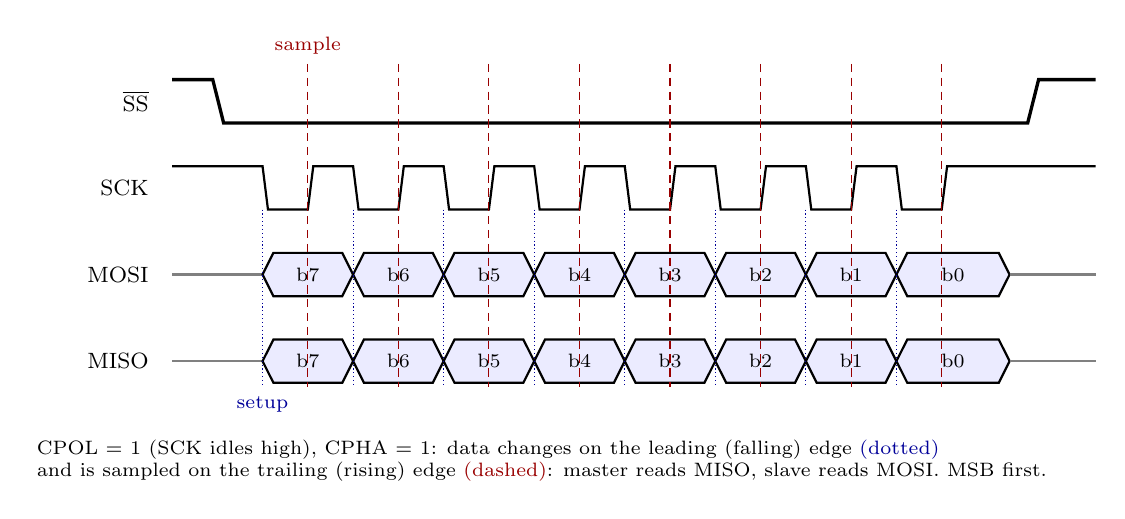
\begin{tikzpicture}[>=Stealth,font=\small,x=1.15cm,y=1cm]
% row 0 y=0
\node[anchor=east,font=\footnotesize,align=right] at (-0.15,0.275) {$\overline{\mathrm{SS}}$};
\draw[very thick] (0,0.55) -- (0.45,0.55) -- (0.57,0) -- (9.45,0) -- (9.57,0.55) -- (10.2,0.55);
% row 1 y=-1.1
\node[anchor=east,font=\footnotesize,align=right] at (-0.15,-0.825) {SCK};
\draw[thick] (0,-0.55) -- (1,-0.55) -- (1.06,-1.1) -- (1.5,-1.1) -- (1.56,-0.55) -- (2,-0.55) -- (2.06,-1.1) -- (2.5,-1.1) -- (2.56,-0.55) -- (3,-0.55) -- (3.06,-1.1) -- (3.5,-1.1) -- (3.56,-0.55) -- (4,-0.55) -- (4.06,-1.1) -- (4.5,-1.1) -- (4.56,-0.55) -- (5,-0.55) -- (5.06,-1.1) -- (5.5,-1.1) -- (5.56,-0.55) -- (6,-0.55) -- (6.06,-1.1) -- (6.5,-1.1) -- (6.56,-0.55) -- (7,-0.55) -- (7.06,-1.1) -- (7.5,-1.1) -- (7.56,-0.55) -- (8,-0.55) -- (8.06,-1.1) -- (8.5,-1.1) -- (8.56,-0.55) -- (10.2,-0.55);
% row 2 y=-2.2
\node[anchor=east,font=\footnotesize,align=right] at (-0.15,-1.925) {MOSI};
\draw[thick,gray] (0,-1.925) -- (1,-1.925);
\draw[thick,fill=blue!8] (1,-1.925) -- (1.12,-1.65) -- (1.88,-1.65) -- (2,-1.925) -- (1.88,-2.2) -- (1.12,-2.2) -- cycle;
\node[font=\scriptsize] at (1.5,-1.925) {b7};
\draw[thick,fill=blue!8] (2,-1.925) -- (2.12,-1.65) -- (2.88,-1.65) -- (3,-1.925) -- (2.88,-2.2) -- (2.12,-2.2) -- cycle;
\node[font=\scriptsize] at (2.5,-1.925) {b6};
\draw[thick,fill=blue!8] (3,-1.925) -- (3.12,-1.65) -- (3.88,-1.65) -- (4,-1.925) -- (3.88,-2.2) -- (3.12,-2.2) -- cycle;
\node[font=\scriptsize] at (3.5,-1.925) {b5};
\draw[thick,fill=blue!8] (4,-1.925) -- (4.12,-1.65) -- (4.88,-1.65) -- (5,-1.925) -- (4.88,-2.2) -- (4.12,-2.2) -- cycle;
\node[font=\scriptsize] at (4.5,-1.925) {b4};
\draw[thick,fill=blue!8] (5,-1.925) -- (5.12,-1.65) -- (5.88,-1.65) -- (6,-1.925) -- (5.88,-2.2) -- (5.12,-2.2) -- cycle;
\node[font=\scriptsize] at (5.5,-1.925) {b3};
\draw[thick,fill=blue!8] (6,-1.925) -- (6.12,-1.65) -- (6.88,-1.65) -- (7,-1.925) -- (6.88,-2.2) -- (6.12,-2.2) -- cycle;
\node[font=\scriptsize] at (6.5,-1.925) {b2};
\draw[thick,fill=blue!8] (7,-1.925) -- (7.12,-1.65) -- (7.88,-1.65) -- (8,-1.925) -- (7.88,-2.2) -- (7.12,-2.2) -- cycle;
\node[font=\scriptsize] at (7.5,-1.925) {b1};
\draw[thick,fill=blue!8] (8,-1.925) -- (8.12,-1.65) -- (9.13,-1.65) -- (9.25,-1.925) -- (9.13,-2.2) -- (8.12,-2.2) -- cycle;
\node[font=\scriptsize] at (8.625,-1.925) {b0};
\draw[thick,gray] (9.25,-1.925) -- (10.2,-1.925);
% row 3 y=-3.3
\node[anchor=east,font=\footnotesize,align=right] at (-0.15,-3.025) {MISO};
\draw[thick,gray] (0,-3.025) -- (1,-3.025);
\draw[thick,fill=blue!8] (1,-3.025) -- (1.12,-2.75) -- (1.88,-2.75) -- (2,-3.025) -- (1.88,-3.3) -- (1.12,-3.3) -- cycle;
\node[font=\scriptsize] at (1.5,-3.025) {b7};
\draw[thick,fill=blue!8] (2,-3.025) -- (2.12,-2.75) -- (2.88,-2.75) -- (3,-3.025) -- (2.88,-3.3) -- (2.12,-3.3) -- cycle;
\node[font=\scriptsize] at (2.5,-3.025) {b6};
\draw[thick,fill=blue!8] (3,-3.025) -- (3.12,-2.75) -- (3.88,-2.75) -- (4,-3.025) -- (3.88,-3.3) -- (3.12,-3.3) -- cycle;
\node[font=\scriptsize] at (3.5,-3.025) {b5};
\draw[thick,fill=blue!8] (4,-3.025) -- (4.12,-2.75) -- (4.88,-2.75) -- (5,-3.025) -- (4.88,-3.3) -- (4.12,-3.3) -- cycle;
\node[font=\scriptsize] at (4.5,-3.025) {b4};
\draw[thick,fill=blue!8] (5,-3.025) -- (5.12,-2.75) -- (5.88,-2.75) -- (6,-3.025) -- (5.88,-3.3) -- (5.12,-3.3) -- cycle;
\node[font=\scriptsize] at (5.5,-3.025) {b3};
\draw[thick,fill=blue!8] (6,-3.025) -- (6.12,-2.75) -- (6.88,-2.75) -- (7,-3.025) -- (6.88,-3.3) -- (6.12,-3.3) -- cycle;
\node[font=\scriptsize] at (6.5,-3.025) {b2};
\draw[thick,fill=blue!8] (7,-3.025) -- (7.12,-2.75) -- (7.88,-2.75) -- (8,-3.025) -- (7.88,-3.3) -- (7.12,-3.3) -- cycle;
\node[font=\scriptsize] at (7.5,-3.025) {b1};
\draw[thick,fill=blue!8] (8,-3.025) -- (8.12,-2.75) -- (9.13,-2.75) -- (9.25,-3.025) -- (9.13,-3.3) -- (8.12,-3.3) -- cycle;
\node[font=\scriptsize] at (8.625,-3.025) {b0};
\draw[thick,gray] (9.25,-3.025) -- (10.2,-3.025);

\foreach \k in {0,...,7} {
  \draw[red!60!black,densely dashed] (1.5+\k,0.75) -- (1.5+\k,-3.35);
  \draw[blue!60!black,densely dotted] (1.0+\k,-1.1) -- (1.0+\k,-3.35);
}
\node[font=\scriptsize,red!60!black,anchor=south] at (1.5,0.75) {sample};
\node[font=\scriptsize,blue!60!black,anchor=north] at (1.0,-3.35) {setup};
\node[font=\scriptsize,align=left,anchor=north west] at (-1.6,-3.9) {CPOL = 1 (SCK idles high), CPHA = 1: data changes on the leading (falling) edge \textcolor{blue!60!black}{(dotted)}\\and is sampled on the trailing (rising) edge \textcolor{red!60!black}{(dashed)}: master reads MISO, slave reads MOSI. MSB first.};

\end{tikzpicture}
\end{document}
